\documentclass[ignorenonframetext,xcolor=x11names]{beamer}

\input{../common.preamble.beamer.tex}

\title{Business 4720 - Class 16}

\subtitle{Convolutional Neural Networks using Python}

\begin{document}

\begin{frame}{}
  \titlepage
  \footnotesize
  \input{../license.tex}
\end{frame}

\section{Introduction}

\begin{frame}{This Class}

\begin{block}{What You Will Learn:}
\begin{itemize}
  \item Deep Learning Concepts
  \begin{itemize}
     \item Convolutional Neural Networks
     \item Text Classification with Neural Networks
  \end{itemize}
\end{itemize}
\end{block}
\end{frame}

\begin{frame}{Based On}
\small
\begin{block}{}
Gareth James, Daniel Witten, Trevor Hastie and Robert Tibshirani: \emph{An Introduction to Statistical Learning with Applications in R}. 2nd edition, corrected printing, June 2023. (ISLR2) \\
\vspace{1mm}
\url{https://www.statlearning.com} \\
\vspace{1mm}
Chapter 10
\end{block}

\begin{block}{}
Kevin P. Murphy: \emph{Probabilistic Machine Learning -- An Introduction}. MIT Press 2022. \\
\vspace{1mm}
\url{https://probml.github.io/pml-book/book1.html} \\
\vspace{1mm}
Chapter 13, 14, 15
\end{block}

\begin{block}{Tensorflow Guides}
\url{https://www.tensorflow.org/guide} \\
\url{https://www.tensorflow.org/tutorials/load_data/text}
\end{block}
\end{frame}

\begin{frame}{Convolutional Neural Networks}
\begin{block}{Task}
\begin{itemize}
   \item Image classification
\end{itemize}
\end{block}
\begin{block}{Problem}
\begin{itemize}
   \item Translation, scaling, and rotation of objects in images
\end{itemize}
\end{block}
\begin{block}{Solution}
\begin{itemize}
   \item Learning low-level and high-level ''features'' by learning a sequence of ''filters'' or ''kernels''
\end{itemize}
\end{block}
\end{frame}

\begin{frame}{Convolution}
\begin{block}{1-Dimensional}
\centering
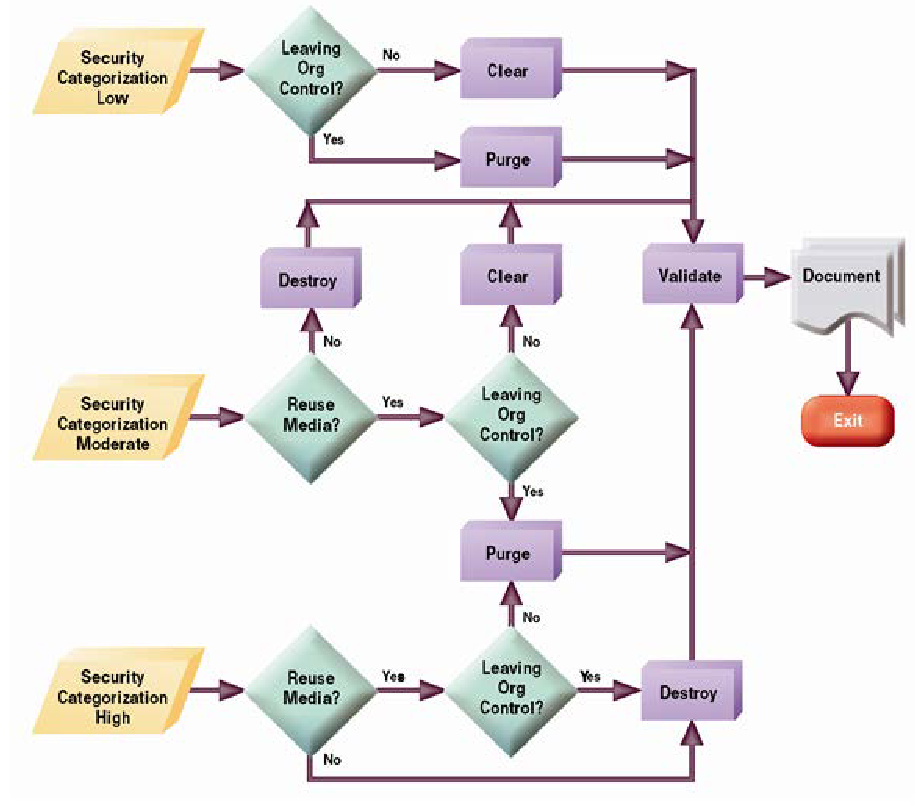
\includegraphics[width=\textwidth]{screen1.png} \\

\scriptsize Source: Murphy Fig. 14.4 \normalsize
\end{block}
\begin{block}{2-Dimensional}
\centering
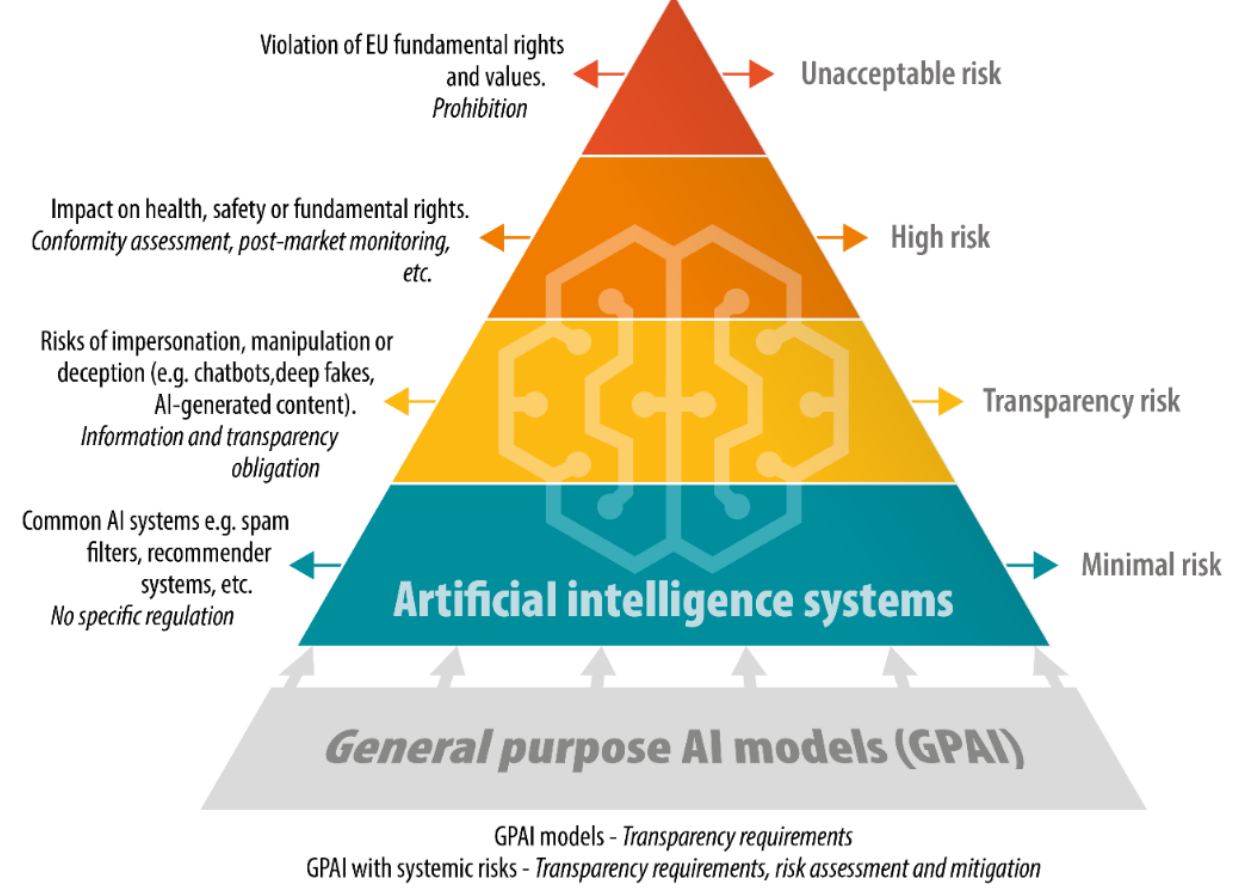
\includegraphics[width=.8\textwidth]{screen2.png} \\

\scriptsize Source: Murphy Fig. 14.5
\end{block}
\end{frame}

\begin{frame}{Convolution \small [cont'd]}
\begin{block}{Multi-channel 2D Convolution}
\centering
\includegraphics[width=.8\textwidth]{screen3.png} \\

\scriptsize Source: Murphy Fig. 14.9
\end{block}
\vspace{\baselineskip}
\emph{In a convolutional neural net layer, the convolution kernels are \textbf{trainable parameters}}.
\end{frame}

\begin{frame}{CNN Parameters}
\small
\begin{itemize}
  \item Let the kernel be of size $k \times l$
  \item Let the input be of $m$ channels
  \item Let the output be $n$ channels
  \item Then, there are $k \times l$ elements for each of the $m$ input dimensions, i.e. a total of $m \times k \times l$
  \item Then, there are $m \times k \times l$ elements for each of the $n$ output dimensions, i.e. a total of $n \times m \times k \times l$
  \item Additionally, there are $n$ bias terms, one for each output channel
\end{itemize}
\textbf{Example}: Let the kernel size be $5 \times 5$ applied to an input with $3$ channels and an output of $32$ channels. Then, the CNN layer has $32 \times 3 \times 5 \times 5 + 32 = 2432$ parameters.
\end{frame}


\begin{frame}{Hands-On Exercises}
Calculate the number of trainable parameters for the following CNN layers:
\begin{enumerate}
\item A kernel of size $4 \times 4$ operating on an input with 3 channels and an output of 8 channels.
\item A kernel of size $2 \times 2$ operating on an input with 8 channels and an output of 16 channels.
\item A kernel of size $3 \times 3$ operating on an input with 16 channels and an output of 4 channels.
\item A kernel of size $5 \times 5$ operating on an input with 4 channels and an output with 4 channels.
\end{enumerate}
Assume the previous four layers are part of the same neural network, what is the total number of trainable parameters?
\end{frame}


\begin{frame}{Convolution \small [cont'd]}{Striding and Padding}
\begin{block}{Striding}
   \begin{itemize} 
       \item Take ''larger steps'' moving the kernel
       \item Remove redundancy
       \item Increase efficiency
   \end{itemize}
\end{block}
\begin{block}{Padding}
   \begin{itemize}
       \item Surround the data matrix by zeros
       \item Increases weight of edge pixels
       \item Allows same-convolution, i.e. output size is the same as input size
   \end{itemize}
\end{block}
\end{frame}

\begin{frame}{Convolution \small [cont'd]}{Striding and Padding}
\centering
\includegraphics[width=.8\textwidth]{screen4.png} \\

\scriptsize Source: Murphy Fig. 14.8(b)
\end{frame}

\begin{frame}{Pooling}
\begin{itemize}
   \item Recognize location independent features
   \item Max pooling or average pooling
   \item Pooling layers have no trainable parameters
\end{itemize}
\centering
\includegraphics[width=.8\textwidth]{screen5.png} \\

\scriptsize Source: Murphy Fig. 14.12
\end{frame}

\begin{frame}{Hands-On Exercises}
\small
\begin{enumerate}
\item Assume the following $5 \times 5$ input matrix:
\begin{align*}
\begin{bmatrix} 1 & 2 & 3 & 2 & 1 \\ 
                2 & 3 & 2 & 1 & 3 \\ 
                3 & 2 & 1 & 3 & 2 \\
                2 & 1 & 3 & 2 & 1 \\               
                1 & 3 & 2 & 1 & 3 
\end{bmatrix}
\end{align*}
and the following $3 \times 3$ convolution kernel:
\begin{align*}
\begin{bmatrix}  1 & 2 & 1 \\ 
                2 & 4 & 2 \\
                1 & 2 & 1 \end{bmatrix}
\end{align*}
Zero-pad the matrix with two zeros on all sides and using stride 2, calculate the convolution result. What are the dimensions of the convolution output?

\item Apply a $2 \times 2$ max pooling layer to the result of the previous exercise. 
\end{enumerate}
\end{frame}




\begin{frame}{CNN}
\begin{itemize}
   \item Multiple convolution and pooling (subsampling) layers
   \item Flatten final feature maps
   \item Multiple fully connected layers
   \item Softmax output
\end{itemize}
\vspace{\baselineskip}
\centering
\includegraphics[width=\textwidth]{screen6.png} \\

\scriptsize Source: Murphy Fig. 14.13
\end{frame}

\begin{frame}{CNN}
\begin{itemize}
   \item Multiple convolutional kernels applied in parallel to the same image (''channels'')
\end{itemize} 

\vspace{\baselineskip}

\centering
\includegraphics[width=\textwidth]{screen12.png} \\
\vspace{\baselineskip}

\hrule

\vspace{\baselineskip}
\scriptsize Source: Matthew D. Zeiler and Rob Fergus (2013) Visualizing and Understanding Convolutional Networks. \url{https://doi.org/10.48550/arXiv.1311.2901}
\end{frame}

\begin{frame}{CNN -- Feature Maps}
\begin{columns}
\begin{column}{0.5\textwidth}
\begin{itemize}
   \item ReLU'd and Pooled Convolution is a ''\textbf{Feature Map}''
   \item Features maps at different layers identify different types of features
   \item Features form the input to the fully connected layers for classification
   \item Visualization e.g. with DeconvNet
\end{itemize}
\end{column}
\begin{column}{0.5\textwidth}
\centering
\includegraphics[width=.95\textwidth]{screen13.png} \\

\vspace{\baselineskip}
\scriptsize Source: Matthew D. Zeiler and Rob Fergus (2013) Visualizing and Understanding Convolutional Networks. \url{https://doi.org/10.48550/arXiv.1311.2901}
\end{column}
\end{columns}
\end{frame}

\begin{frame}{CNN -- Feature Maps}
\centering
\includegraphics[height=2in]{layer1.png} \\
\vspace{\baselineskip}
\scriptsize Source: Matthew D. Zeiler and Rob Fergus (2013) Visualizing and Understanding Convolutional Networks. \url{https://doi.org/10.48550/arXiv.1311.2901}
\end{frame}

\begin{frame}{CNN -- Feature Maps}
\centering
\includegraphics[height=2in]{layer2.png} \\
\vspace{\baselineskip}
\scriptsize Source: Matthew D. Zeiler and Rob Fergus (2013) Visualizing and Understanding Convolutional Networks. \url{https://doi.org/10.48550/arXiv.1311.2901}
\end{frame}

\begin{frame}{CNN -- Feature Maps}
\centering
\includegraphics[width=\textwidth]{layer3.png} \\
\vspace{\baselineskip}
\scriptsize Source: Matthew D. Zeiler and Rob Fergus (2013) Visualizing and Understanding Convolutional Networks. \url{https://doi.org/10.48550/arXiv.1311.2901}
\end{frame}

\begin{frame}{CNN -- Feature Maps}
\centering
\includegraphics[height=2.75in]{layers45.png} \\
\vspace{0.5\baselineskip}
\scriptsize Source: Matthew D. Zeiler and Rob Fergus (2013) Visualizing and Understanding Convolutional Networks. \url{https://doi.org/10.48550/arXiv.1311.2901}
\end{frame}

\begin{frame}{CNN in Keras}
\centering
\includegraphics[height=2in]{cifar10.png}
\begin{itemize}
   \item 60,000 images, $32 \times 32$ resolution, 3 channels
   \item 10 classes
   \item Latest error rate $< 0.5\%$
\end{itemize}
\end{frame}

\begin{frame}[fragile]{CNN in Keras}
Import the data:
\begin{pythoncode}
import tensorflow as tf
from tensorflow.keras import datasets, layers, models
import datetime

(train_images, train_labels), (test_images, test_labels) \
    = datasets.cifar10.load_data()

# Normalize pixel values to be between 0 and 1
train_images = train_images / 255.0
test_images = test_images / 255.0
\end{pythoncode}
Show sample images:
\begin{pythoncode}
import plotly
import plotly.express as px

fig = plotly.subplots.make_subplots(rows=5, cols=5)
for i in range(25):
    fig.add_trace(px.imshow(train_images[i]).data[0], 
                            row=i//5+1, col=i%5+1)
fig.show()
\end{pythoncode}
\end{frame}

\begin{frame}[fragile]{CNN in Keras}
Create a simple convolutional model:
\begin{pythoncode}
model = models.Sequential()

model.add(layers.Conv2D(8, (3, 3), activation='relu', \
    input_shape=(32, 32, 3)))
model.add(layers.MaxPooling2D((2, 2)))

model.add(layers.Conv2D(16, (3, 3), activation='relu'))
model.add(layers.MaxPooling2D((2, 2)))

model.add(layers.Conv2D(16, (3, 3), activation='relu'))
\end{pythoncode}
Add dense (fully-connected) layers for classification. There are 10 target classes:
\begin{pythoncode}
model.add(layers.Flatten())
model.add(layers.Dense(32, activation='relu'))
model.add(layers.Dense(10))

model.summary()
\end{pythoncode}
\end{frame}

\begin{frame}[fragile]{CNN in Keras}
Compile and train the model:
\begin{pythoncode}
model.compile(
    optimizer='adam',
    loss=tf.keras.losses \
        .SparseCategoricalCrossentropy(from_logits=True),
    metrics=['accuracy'])

model.fit(
    train_images, train_labels, epochs=10, 
    validation_data=(test_images, test_labels))
\end{pythoncode}
\end{frame}

\begin{frame}{Other Computer Vision Tasks for CNNs}{Object Detection}
\includegraphics[width=\textwidth]{screen10.png} \\

\scriptsize Source: Murphy Fig. 14.27
\normalsize
\begin{align*}
f_\theta: R^{H\times W \times K} \rightarrow [0,1]^{A \times A} \times \{1, \ldots, C\}^{A \times A} \times (R^4)^{A \times A}
\end{align*}
For each anchor box, learn the object presence probability, the object category and two offset vectors to be added to the center of the box to the top left and bottom right corners.
\end{frame}

\begin{frame}{Other Computer Vision Tasks for CNNs}{Semantic Segmentation}
\includegraphics[width=\textwidth]{screen11.png} \\

\scriptsize Source: Murphy Fig. 14.29
\normalsize
\vspace{\baselineskip}

Using an \textbf{encoder-decoder} or \textbf{U-net} network to identify the class of each pixel in an image.
\end{frame}

\begin{frame}{Other Computer Vision Tasks for CNNs}
\begin{center}
\includegraphics[width=.5\textwidth]{street.png} \\

\scriptsize \url{https://github.com/matterport/Mask_RCNN}
\end{center}

\normalsize
Perform semantic segmentation within each anchor box from object detection to identify foreground (object) and background. 
\end{frame}


\begin{frame}[fragile]{Text Classification using CNN}
Import packages:
\begin{pythoncode}
import collections
import pathlib
import datetime

import tensorflow as tf
from tensorflow.keras import layers
from tensorflow.keras import losses
from tensorflow.keras import utils
from tensorflow.keras.layers import TextVectorization
\end{pythoncode}
\end{frame}

\begin{frame}[fragile]{Text Classification using NN \small [cont'd]}
Download the Stack Overflow dataset:
\begin{pythoncode}
data_url = \
'http://download.tensorflow.org/data/stack_overflow_16k.tar.gz'

# Get the data
dataset_dir = utils.get_file(origin=data_url, untar=True,
               cache_subdir='stack_overflow')

# Remember where we put it
dataset_dir = pathlib.Path(dataset_dir).parent
train_dir = dataset_dir/'train'
test_dir = dataset_dir/'test'

# Print a sample
sample_file = train_dir/'python/1755.txt'
with open(sample_file) as f:
    print(f.read())
\end{pythoncode}
\end{frame}


\begin{frame}[fragile]{Text Classification using NN \small [cont'd]}
\centering

\includegraphics[width=.8\textwidth]{screen9.png}
\end{frame}

\begin{frame}[fragile]{Text Classification using NN \small [cont'd]}
Read the training data portion and split into training and validation set
\begin{pythoncode}
raw_train_ds = \
utils.text_dataset_from_directory(
    train_dir, batch_size=32,
    validation_split=0.2,
    subset='training', seed=42)
    
raw_val_ds = \
utils.text_dataset_from_directory(
    train_dir, batch_size=32,
    validation_split=0.2,
    subset='validation', seed=42)
\end{pythoncode}
Read the test set portion of the dataset:
\begin{pythoncode}
raw_test_ds = utils.text_dataset_from_directory(
    test_dir, batch_size=32)
\end{pythoncode}
\end{frame}

\begin{frame}[fragile]{Text Classification using NN \small [cont'd]}
\begin{block}{Pre-Processing}
\begin{itemize}
   \item \textbf{Standardization}: Remove punction, remove HTML elements, etc.
   \item \textbf{Tokenization}: Split strings to tokens (e.g. sentences into words on whitespace)
   \item \textbf{Vectorization}: Convert tokens into numbers for input into a neural network
\end{itemize}
\end{block}
\begin{block}{Bag-of-Word Model}
\begin{itemize}
   \item Counts frequency of words/tokens
   \item Neglects order
\end{itemize}
\begin{textcode}
John likes to watch movies. Mary likes movies too.
{"John":1,"likes":2,"to":1,"watch":1,
 "movies":2,"Mary":1,"too":1}
\end{textcode}
\end{block}
\end{frame}


\begin{frame}[fragile]{Text Classification Using NN \small [cont'd]}
Use the Keras \texttt{TextVectorization} pre-processing layer:
\begin{pythoncode}
multi_hot_vectorize_layer = TextVectorization(
    max_tokens=10000,
    standardize='lower_and_strip_punctuation',
    split='whitespace',
    output_mode='multi_hot')
    
# Get only the text from the training set
train_text = raw_train_ds.map(lambda text,labels: text)
multi_hot_vectorize_layer.adapt(train_text)
\end{pythoncode}
\end{frame}


\begin{frame}[fragile]{Text Classification Using NN \small [cont'd]}
\begin{itemize}
   \item The ''multi-hot'' vectorization layer outputs a single integer array per mini-batch, containing 1s in all elements where the token mapped to that index exists at least once in the mini-batch item. 
\end{itemize}

\begin{pythoncode}
# Retrieve a batch from the dataset
text_batch, label_batch = next(iter(raw_train_ds))

# Applying the text vectorization layer 
# to the first example and print its output
print(text_batch[0])
print(list(multi_hot_vectorize_layer(text_batch[0]).numpy()))
\end{pythoncode}
\end{frame}

\begin{frame}[fragile]{Text Classification Using NN \small [cont'd]}
Define a simple model, set loss function, optimizer and a metric to collect:
\begin{pythoncode}
multi_hot_model = tf.keras.Sequential([
    multi_hot_vectorize_layer,
    layers.Dense(4)])

multi_hot_model.compile(
    loss= \
      losses.SparseCategoricalCrossentropy(from_logits=True),
    optimizer='adam',
    metrics=['accuracy'])
\end{pythoncode}
\end{frame}

\begin{frame}[fragile]{Text Classification Using NN \small [cont'd]}
Train the model for 25 epochs, showing validation set accuracy after each epoch:
\begin{pythoncode}
multi_hot_model.fit(raw_train_ds, 
                    validation_data=raw_val_ds, 
                    epochs=25)
\end{pythoncode}
\end{frame}

\begin{frame}{Hands-On Exercises}
Adapt the network architecture to identify the impact on training and validation performance of the following:
   \begin{enumerate}
      \item Vocabulary size (originally 10 000)
      \item Number of layers (originally 1)
   \end{enumerate}
Comment on your findings and identify the best model.
\end{frame}


\begin{frame}[fragile]{Text Classification Using CNN \small [cont'd]}
Use the Keras \texttt{TextVectorization} pre-processing layer, this time with integer outputs:
\begin{pythoncode}
int_vectorize_layer = TextVectorization(
    max_tokens=10000,
    standardize='lower_and_strip_punctuation',
    split='whitespace',
    output_mode='int')
    
# Get only the text from the training set
train_text = raw_train_ds.map(lambda text,labels: text)
# Adapt the layer
int_vectorize_layer.adapt(train_text)
\end{pythoncode}
\end{frame}


\begin{frame}[fragile]{Text Classification Using CNN \small [cont'd]}
\begin{itemize}
   \item The ''int'' vectorization layer outputs integer indices, one integer index per split string token. 
\end{itemize}

\begin{pythoncode}
# Retrieve a batch from the dataset
text_batch, label_batch = next(iter(raw_train_ds))

# Applying the text vectorization layer 
# to the first example and print its output
print(text_batch[0])
print(list(int_vectorize_layer(text_batch[0]).numpy()))
\end{pythoncode}
\end{frame}

\begin{frame}{Word Embeddings}
\begin{columns}
\begin{column}{.5\textwidth}
\includegraphics[width=\textwidth]{one-hot.png}
\end{column}
\begin{column}{.5\textwidth}
\includegraphics[width=\textwidth]{embedding2.png}
\end{column}
\end{columns}
\begin{center}
\vspace{\baselineskip}
\scriptsize \url{https://www.tensorflow.org/text/guide/word_embeddings}\normalsize
\vspace{\baselineskip}
\end{center}
\begin{itemize}
   \item Embedding matrix elements are \textbf{learnable parameters}
   \item Dimension reduction
   \item May be useful to measure similarity of terms
\end{itemize}
\end{frame}


\begin{frame}[fragile]{Text Classification Using NN \small [cont'd]}
Define a 1D-CNN model, set loss function, optimizer and a metric to collect:
\begin{pythoncode}
int_model = tf.keras.Sequential([
  int_vectorize_layer, 
  layers.Embedding(10001, 64, mask_zero=True),
  layers.Dropout(0.5),
  layers.Conv1D(filters=64, kernel_size=5, \
      padding="valid", activation="relu", strides=2),
  layers.GlobalMaxPooling1D(),
  layers.Dense(4)
  ])

int_model.compile(
    loss= \
losses.SparseCategoricalCrossentropy(from_logits=True),
    optimizer='adam',
    metrics=['accuracy'])
\end{pythoncode}
\end{frame}

\begin{frame}[fragile]{Text Classification Using NN \small [cont'd]}
Train the model for 25 epochs:

\begin{pythoncode}
int_model.fit(raw_train_ds, 
              validation_data=raw_val_ds, 
              epochs=25)
\end{pythoncode}
\end{frame}

\begin{frame}{Hands-On Exercises}
Adapt the network architecture to identify the impact on training and validation performance of the following:
   \begin{enumerate}
      \item Vocabulary size (originally 10 000)
      \item Embedding size (originally 64)
      \item Dropout probability (originally 0.5)
      \item Convolution kernel size (originally 5)
      \item Number of convolution filters (originally 64)
      \item Convolution stride (originally 2)
      \item Number of 1D-Conv layers (originally 1)
   \end{enumerate}
Comment on your findings and identify the best model.
\end{frame}

\end{document}



